%!TEX root = mcmpaper.tex
\section{problem b model design}
premise: In order to better measure our optimization effect, we introduce two parameters: queuing satisfaction, and cost effect.As explained below:

\begin{equation}
\left.
\begin{aligned}[b]
  P = \frac{1}{L*S}\footnotemark[1]
\end{aligned}
\right.
\end{equation}

\begin{equation}
\left.
\begin{aligned}[b]
  C=\frac{A_{t}}{A_{0}}+\frac{B_{t}}{B_{0}}
  \footnotemark[2]
\end{aligned}
\right.
\end{equation}

\footnotetext[1]{
	\textbf{P}: Queuing satisfaction\\ 
	\textbf{L}: The time required to pass all security checks;\\ 
	\textbf{S}: The standard deviation of the security period;
}

\footnotetext[2]{
	\textbf{$A_{0}$}: The initial state of the equipment personnel in zone A;\\ 
	\textbf{$A_{t}$}: Improved zone A's equipment personnel;\\ 
	\textbf{$B_{0}$}: The initial state of the equipment personnel in zone B;\\
	\textbf{$B_{t}$}: TImproved zone B's equipment personnel;
}

\subsection{Improve 1}
On the basis of Problem 1, we have recognized the bottleneck. In order to further improve the airport security throughput and reduce the waiting time difference, we first thought is to improve the security process of the zone A . As shown in the title, passengers waiting in zone A for identity verification are inspected at two locations, the travelers using the Pre-Check process and regular travelers. But for the process of identity verification, the use of Pre-Check process or not is not affected. So in order to make full use of each verification entrance of zone A, we cancel the respective queuing of passengers in zone A, and change to uniform distribution queuing.

\subsection{Improve 2}
Secondly, we need to adjust the number of security lanes ratio of every security zone. By the traversal adjustment of regional security lanes in a certain range of the number, we can get the time and its variance spent by travelers in each case. Considering the cost, from which to choose the best ratio.
\par
For this reason, we have made the following improvements to the program of Model 1:
Zone A, B, and C in the simulation program have a processing queue that can be resized. In this question, in order to simulate the number of different inspection lanes, we continue to adjust the parameters for ergodic solution, while running the script than the data obtained, and finally get the best combination.
\par
The result is as followed (Where X-axis represents the number of staff and equipment in zone A, and Y-axis represents the number of staff and equipment in zone B equipment.)

\begin{figure}[H]
\centering
\subfigure[The average time normal passenger spent on security checks] { \label{fig:Waiting_Total}
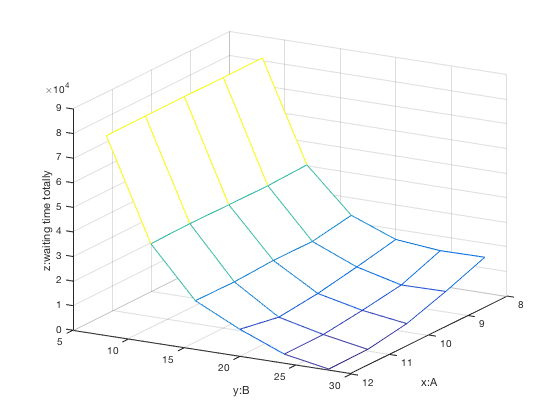
\includegraphics[width=6cm,height=6cm]{/Pic/waiting_total.png}
}
\subfigure[The standard deviation of the time spent on security checks] { \label{fig:waiting_total_std}
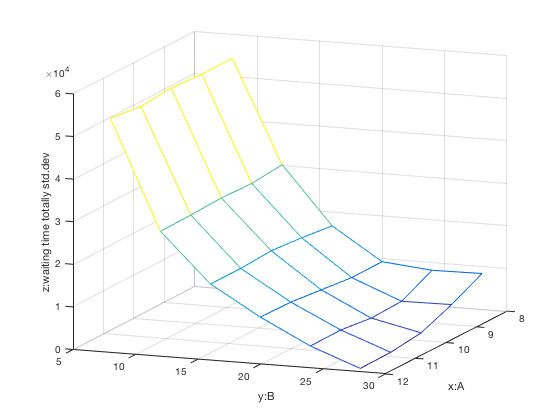
\includegraphics[width=6cm,height=6cm]{/Pic/waiting_tatally_stddev.png}
}
\subfigure[The average time passenger spent on screening with the pre-check passages] { \label{fig:pre_waiting_total}
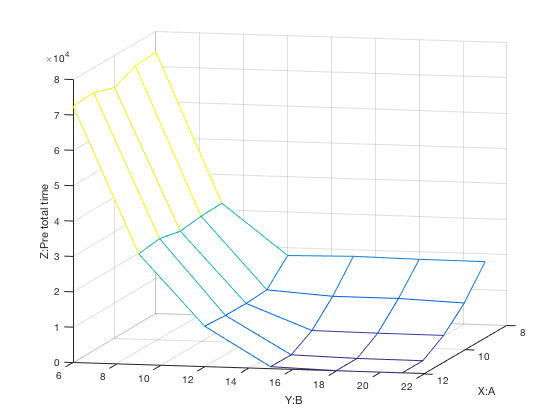
\includegraphics[width=6cm,height=6cm]{/Pic/pre_total_time.png}
}
\subfigure[The standard deviation of the time on screening with the pre-check passages] { \label{fig:pre_waiting_total_std}
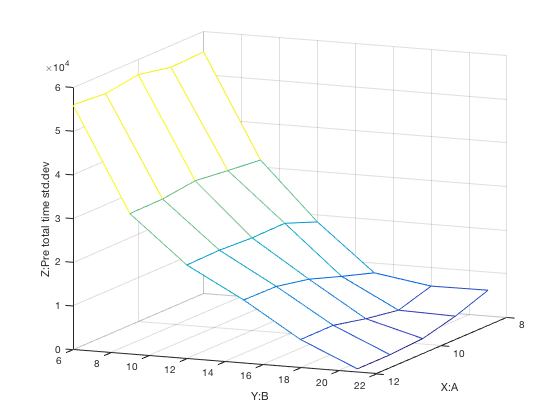
\includegraphics[width=6cm,height=6cm]{/Pic/pre_total_time_stddev.png}
}
\subfigure[The average time spent by all passenger] { \label{fig:pre_waiting_total_std}
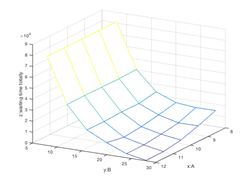
\includegraphics[width=6cm,height=6cm]{/Pic/7.png}
}
\subfigure[The standard deviation of the time spent by all passenger] { \label{fig:total_std}
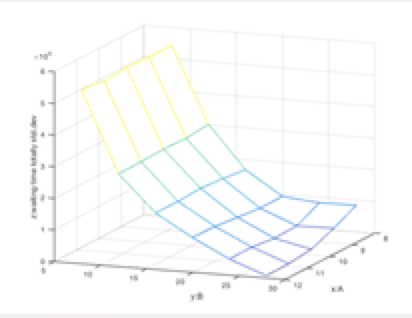
\includegraphics[width=6cm,height=6cm]{/Pic/8.png}
}
\caption{Figures}
\label{fig:Figures}
\end{figure}

According to the figure, with the increase in the number of workers in zone B, both the time-averaged and variance, there is a decreasing trend, that is, the improvement of queuing satisfaction. But when the number increased to a certain extent, the queuing satisfaction index will no longer be significantly improved, but tends to be stable, while the cost effect will still increase fast. Considering two factors, we take the number when the number of staff and equipment in zone A\&B increased to the average time spent and its variance began to change gently. As the optimized number of equipment staff ratio. That is, about 11 sets of equipment and staff in zone A checking identity information, and in zone B the equipment and staff checking belongings and body, for ordinary passengers, 18 sets, for the use of pre-inspection of passengers with 6 sets.( 3: 1 ratio of the information given from the title).

\subsection{Improve 3}
In addition to the above optimization transformation, we can also work on the internal security transformation process. Such as in the most congested zone B, We take into account that the majority of the time is spent on the inspection of the passengers by the staff, and the belongings is checked by the conveyor belt at a reliable speed. So we can on the basis of in each of the original conveyor belt is equipped with one staff checking body, add staff to the side of the belt to improve the efficiency of the zone B, and shorten the time. In order to reflect the optimization results, we may wish to assume that the number of B to add staff, to make the average time in the B zone inspection decreased by 20\%. After that we run the script again, the results are as followed:

\begin{figure}[H]
\centering
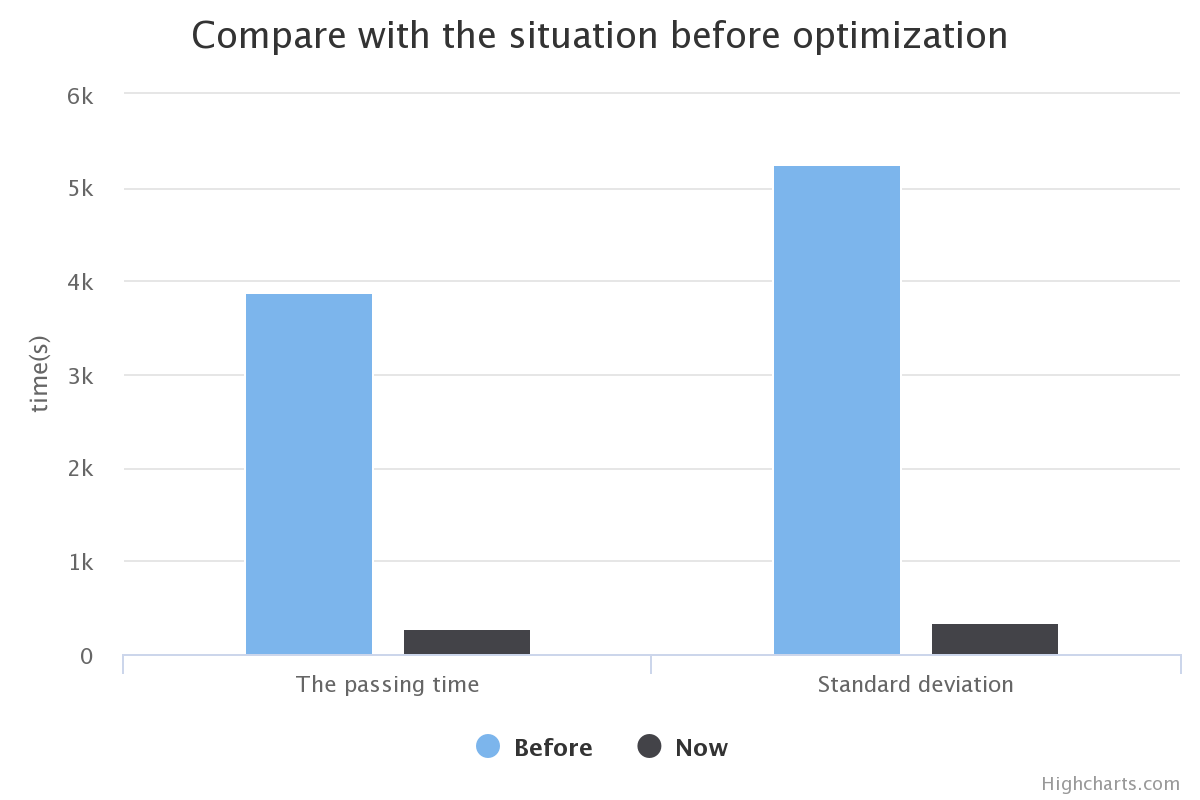
\includegraphics[width=14cm,height=8cm]{/Pic/缩短百分之二十的优化图.png}
\caption{Compare with the situation before optimization}\label{fig:Compare_Pic}
\end{figure}


According to the above figure, the appropriate number of staff to add in zone B can significantly improve work efficiency, reduce the time spent by passengers, improve passenger queuing satisfaction index.









